
\section*{Introduction}
Ce chapitre pose les fondations du projet en présentant le contexte organisationnel et technique de sa réalisation. Après la présentation de \textbf{SolidWall Consulting}, entreprise d'accueil du stage, nous analysons les processus actuels de gestion de maintenance et leurs limitations. L'étude comparative des solutions du marché permet d'identifier les axes d'amélioration et de définir les contours de \textbf{SolidMaint}. Enfin, nous exposons la méthodologie Scrum, le langage UML et la planification prévisionnelle du développement.

\section{Présentation de l’organisme d’accueil} 
« Solid Wall Consulting est une société de services informatiques, spécialisée dans le développement web, le développement mobile et l'intégration de solutions et d'infrastructures systèmes « Microsoft ». 
Forte d'une équipe dynamique et diversifiée et de profils reconnus, l’entreprise a pour objectif constant d'apporter une forte valeur ajoutée et de proposer des solutions modernes permettant aux entreprises de se démarquer sur leurs marchés respectifs. » \cite{site-solidwall} « Fondée avec la vision d'accompagner les organisations publiques et privées vers l'excellence technologique et opérationnelle, Solid Wall Consulting s'est rapidement imposée comme un partenaire de confiance à l'international. » \cite{linkedin-solidwall}.

\begin{figure}[H]
        \centering
        
\includegraphics[width=0.3\textwidth,keepaspectratio]{Images/SolidWall.png}
        \caption{Logo SolidWall Consulting}
        \label{fig:Logo SolidWall Consulting}
\end{figure}

\subsection{ Services de SolidWall Consulting}
\textbf{SolidWall Consulting} est une société spécialisée dans les services informatiques et le développement numérique. Elle accompagne ses clients dans la réussite de leurs projets technologiques en privilégiant une approche agile, ce qui lui permet d'optimiser la gestion de ses prestations et de garantir des solutions modernes, performantes et à forte valeur ajoutée. \cite{site-solidwall}

\newpage
\section{Cadre du projet}
\label{sec:cadre_projet}
Cette partie présente le contexte général du projet et l'étude de l'existant, au niveau interne et international, afin de justifier la solution proposée.
\subsection{Contexte du projet}
Dans le cadre de notre projet de fin d’études (PFE) à l’\textbf{Institut Supérieur des Études Technologiques de Radès} (ISET), nous avons effectué un stage de quatre mois au sein de \textbf{SolidWall Consulting}, du 02 février au 31 mai 2026.
Notre mission consiste à concevoir et à réaliser une application web de gestion des contrats de maintenance.
\newline
Cette solution vise à automatiser et à centraliser l’ensemble du processus métier, garantissant ainsi une traçabilité complète des interventions techniques ainsi que le respect rigoureux des engagements contractuels.

% === CHAPITRE 1 : ANALYSE DE L'EXISTANT ===
\subsection{Analyse de l'existant}
Pour mieux comprendre les besoins, nous allons étudier les solutions existantes à deux niveaux : celles déjà en place au sein de l'entreprise \textbf{SolidWall Consulting}, puis celles utilisées dans le monde.
\subsubsection{Étude de l'existant}
L'étude de l'existant constitue une étape fondamentale de notre démarche projet. Elle permet d'identifier les processus actuels, d'analyser leurs limitations et de définir les axes d'amélioration nécessaires pour concevoir une solution adaptée aux besoins de SolidWall Consulting.
\begin{enumerate}[label=\textcolor{bleuPerso}{\alph*)}, labelsep=0.5em]
            \item   \textcolor{bleuPerso} {Étude de l'existant au niveau de l'entreprise}~\newline
            \noindent
            --\hspace{0.5cm} \textbf{Processus de gestion des contrats de maintenance }
            \newline
            L'entreprise utilise actuellement des documents Word  pour stocker et suivre les informations relatives aux contrats. Ces documents permettent aux responsables de formaliser la relation contractuelle avec les clients et de définir les engagements de chaque partie concernant les services de maintenance.

            Afin de mieux illustrer ce mode de fonctionnement, la figure ci-dessous présente des exemples de gestion des contrats de maintenance dans le système actuel.
            
            \begin{figure}[H]
                \centering
                \begin{subfigure}[b]{0.45\textwidth}
                    \centering
                    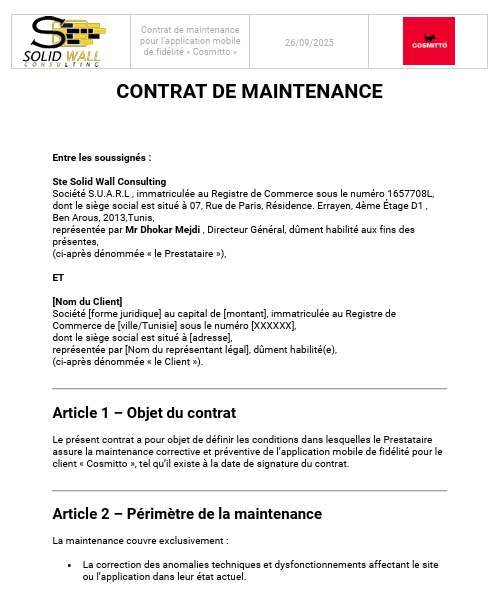
\includegraphics[width=\textwidth, keepaspectratio]{Images/Contrat1.png}
                    
                    \label{fig:contrat1}
                \end{subfigure}
                \hfill
                \begin{subfigure}[b]{0.45\textwidth}
                    \centering
                    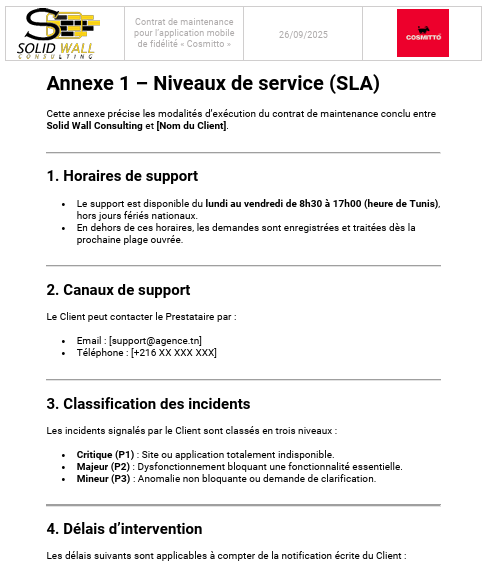
\includegraphics[width=\textwidth, keepaspectratio]{Images/contra2.png}
                    \label{fig:contrat2}
                \end{subfigure}
                \caption{Exemples de contrats de maintenance dans le système actuel}
                \label{fig:exemples_contrats}
            \end{figure}
            \noindent
            --\hspace{0.5cm} \textbf{Processus de gestion des demandes clients }
            \newline
            Le processus des demandes de maintenance repose actuellement sur des échanges via WhatsApp, des messageries instantanées ou des appels téléphoniques. Lorsque le client souhaite signaler un problème, il envoie un message décrivant sa demande au responsable concerné.
           \newline Afin de mieux illustrer ce mode de fonctionnement, la figure ci-dessous présente un exemple de traitement des demandes clients dans le système actuel.
            \begin{figure}[H]
   
    
    
        \centering
        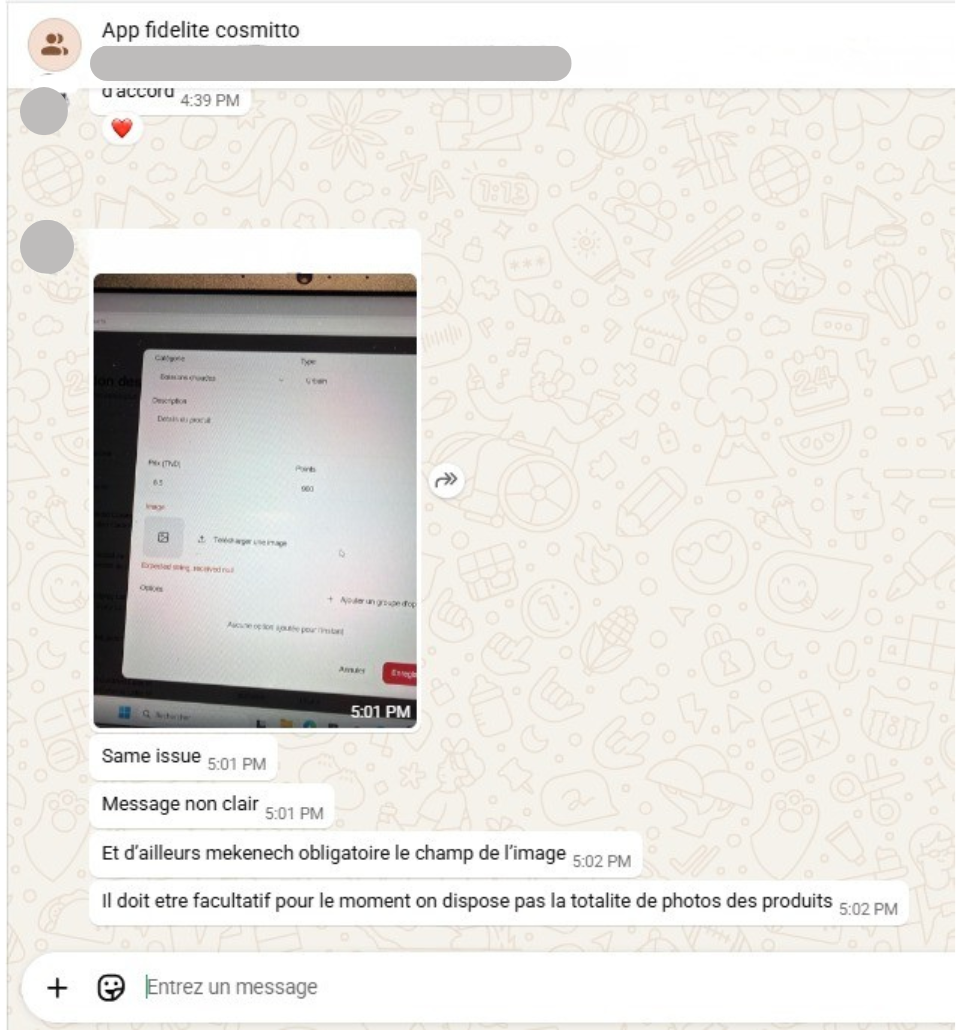
\includegraphics[width=0.40\linewidth, height=0.40\textheight, keepaspectratio]{Images/demande de maintenance.png}
        \caption{Demande de maintenance effectuée via l’application WhatsApp}
        \label{subfig:Demande de maintenance effectuée via l’application WhatsApp}
    \hfill

\end{figure}
\newpage
            \noindent
            --\hspace{0.5cm} \textbf{Processus de suivi des tickets de maintenance }
            \newline
Le suivi des interventions repose au quotidien sur des fils de discussion par e-mail, et l’affectation des tickets aux développeurs est assurée par le responsable, généralement via un message direct. 
\newline Afin d’illustrer plus concrètement ce processus, un exemple de rapport de test et de suivi des anomalies, consigné dans un fichier Excel où sont répertoriés les modules touchés, la description des problèmes rencontrés et leur statut, est présenté ci-dessous.
\begin{figure}[H]
    \centering
    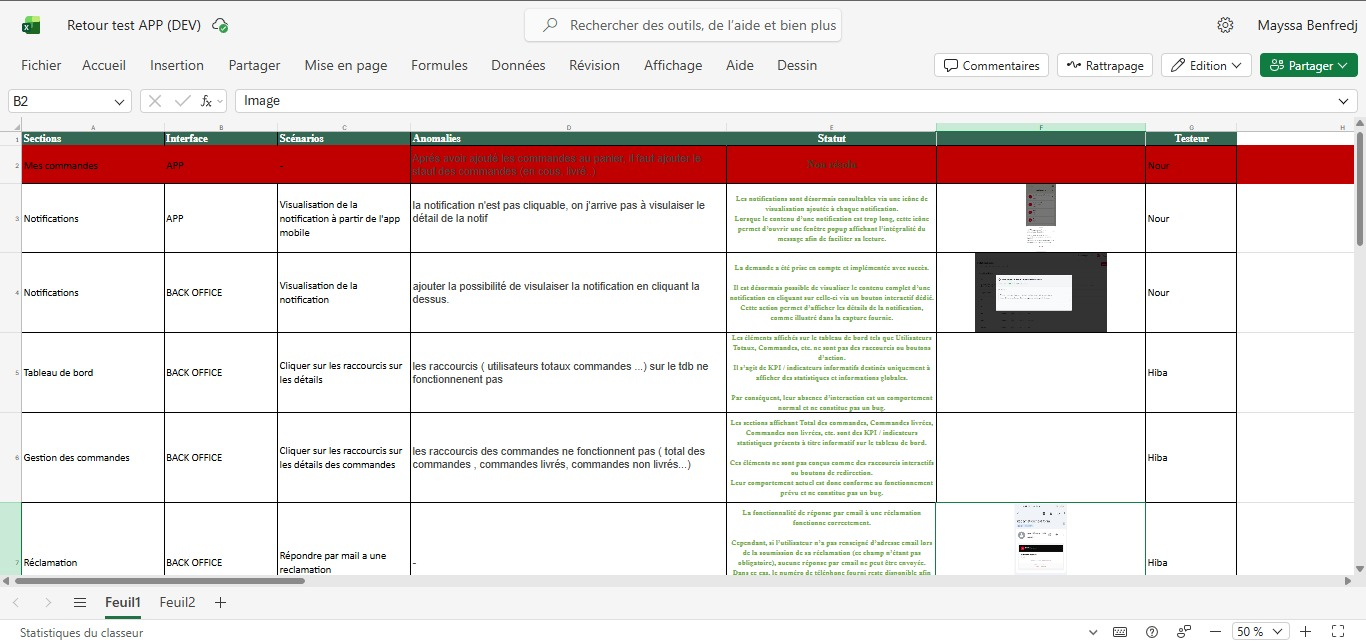
\includegraphics[width=0.80\textwidth, height=0.98\textheight, keepaspectratio]{Images/demande de maintenance sous format excel.png}
    \caption{Exemple de suivi des interventions à l’aide d’un fichier Excel}
    \label{subfig:excel}
\end{figure}
            --\hspace{0.5cm} \textbf{Processus de traçabilité des actions et des documents }
 \newline Les documents contractuels sont stockés dans des répertoires locaux ou sur des espaces de stockage cloud. Les fichiers sont organisés selon les pratiques de chaque responsable, et les modifications sont effectuées directement sur les documents existants.
            \newline

    \item  \textcolor{bleuPerso} {Étude de l'existant à l'échelle internationale}~\newline
            Avant de développer notre propre solution, nous allons étudier les solutions disponibles sur le marché afin d'analyser les fonctionnalités proposées. Cette démarche permet d'identifier les bonnes pratiques et d'orienter efficacement le développement de notre système.\newline
            Dans ce cadre, nous avons étudié plusieurs solutions existantes couvrant différents segments du marché : solutions open-source, solutions \textbf{SaaS} (\textit{Software as a Service}) et solutions enterprise.
\newpage
\noindent  --\hspace{0.5cm}  \textbf{GLPI (Gestionnaire Libre de Parc Informatique)}\par\smallskip
GLPI, lancée en 2003 et maintenue par l’éditeur français Teclib, est une solution open-source de référence pour la gestion des services informatiques et des infrastructures. Elle permet de gérer le parc informatique avec inventaire, licences et cycle de vie des actifs, tout en offrant un centre de services pour le traitement des incidents et des demandes, le suivi des SLA et le maintien d’une base de connaissances conforme aux bonnes pratiques \textbf{ITSM} (\textit{Information Technology Service Management}). La version communautaire est gratuite en on-premise sous licence GPLv3+, tandis que des abonnements payants sont disponibles pour un support cloud managé ou une assistance professionnelle. \cite{glpi} 
                    \begin{figure}[H]
                            \centering
                            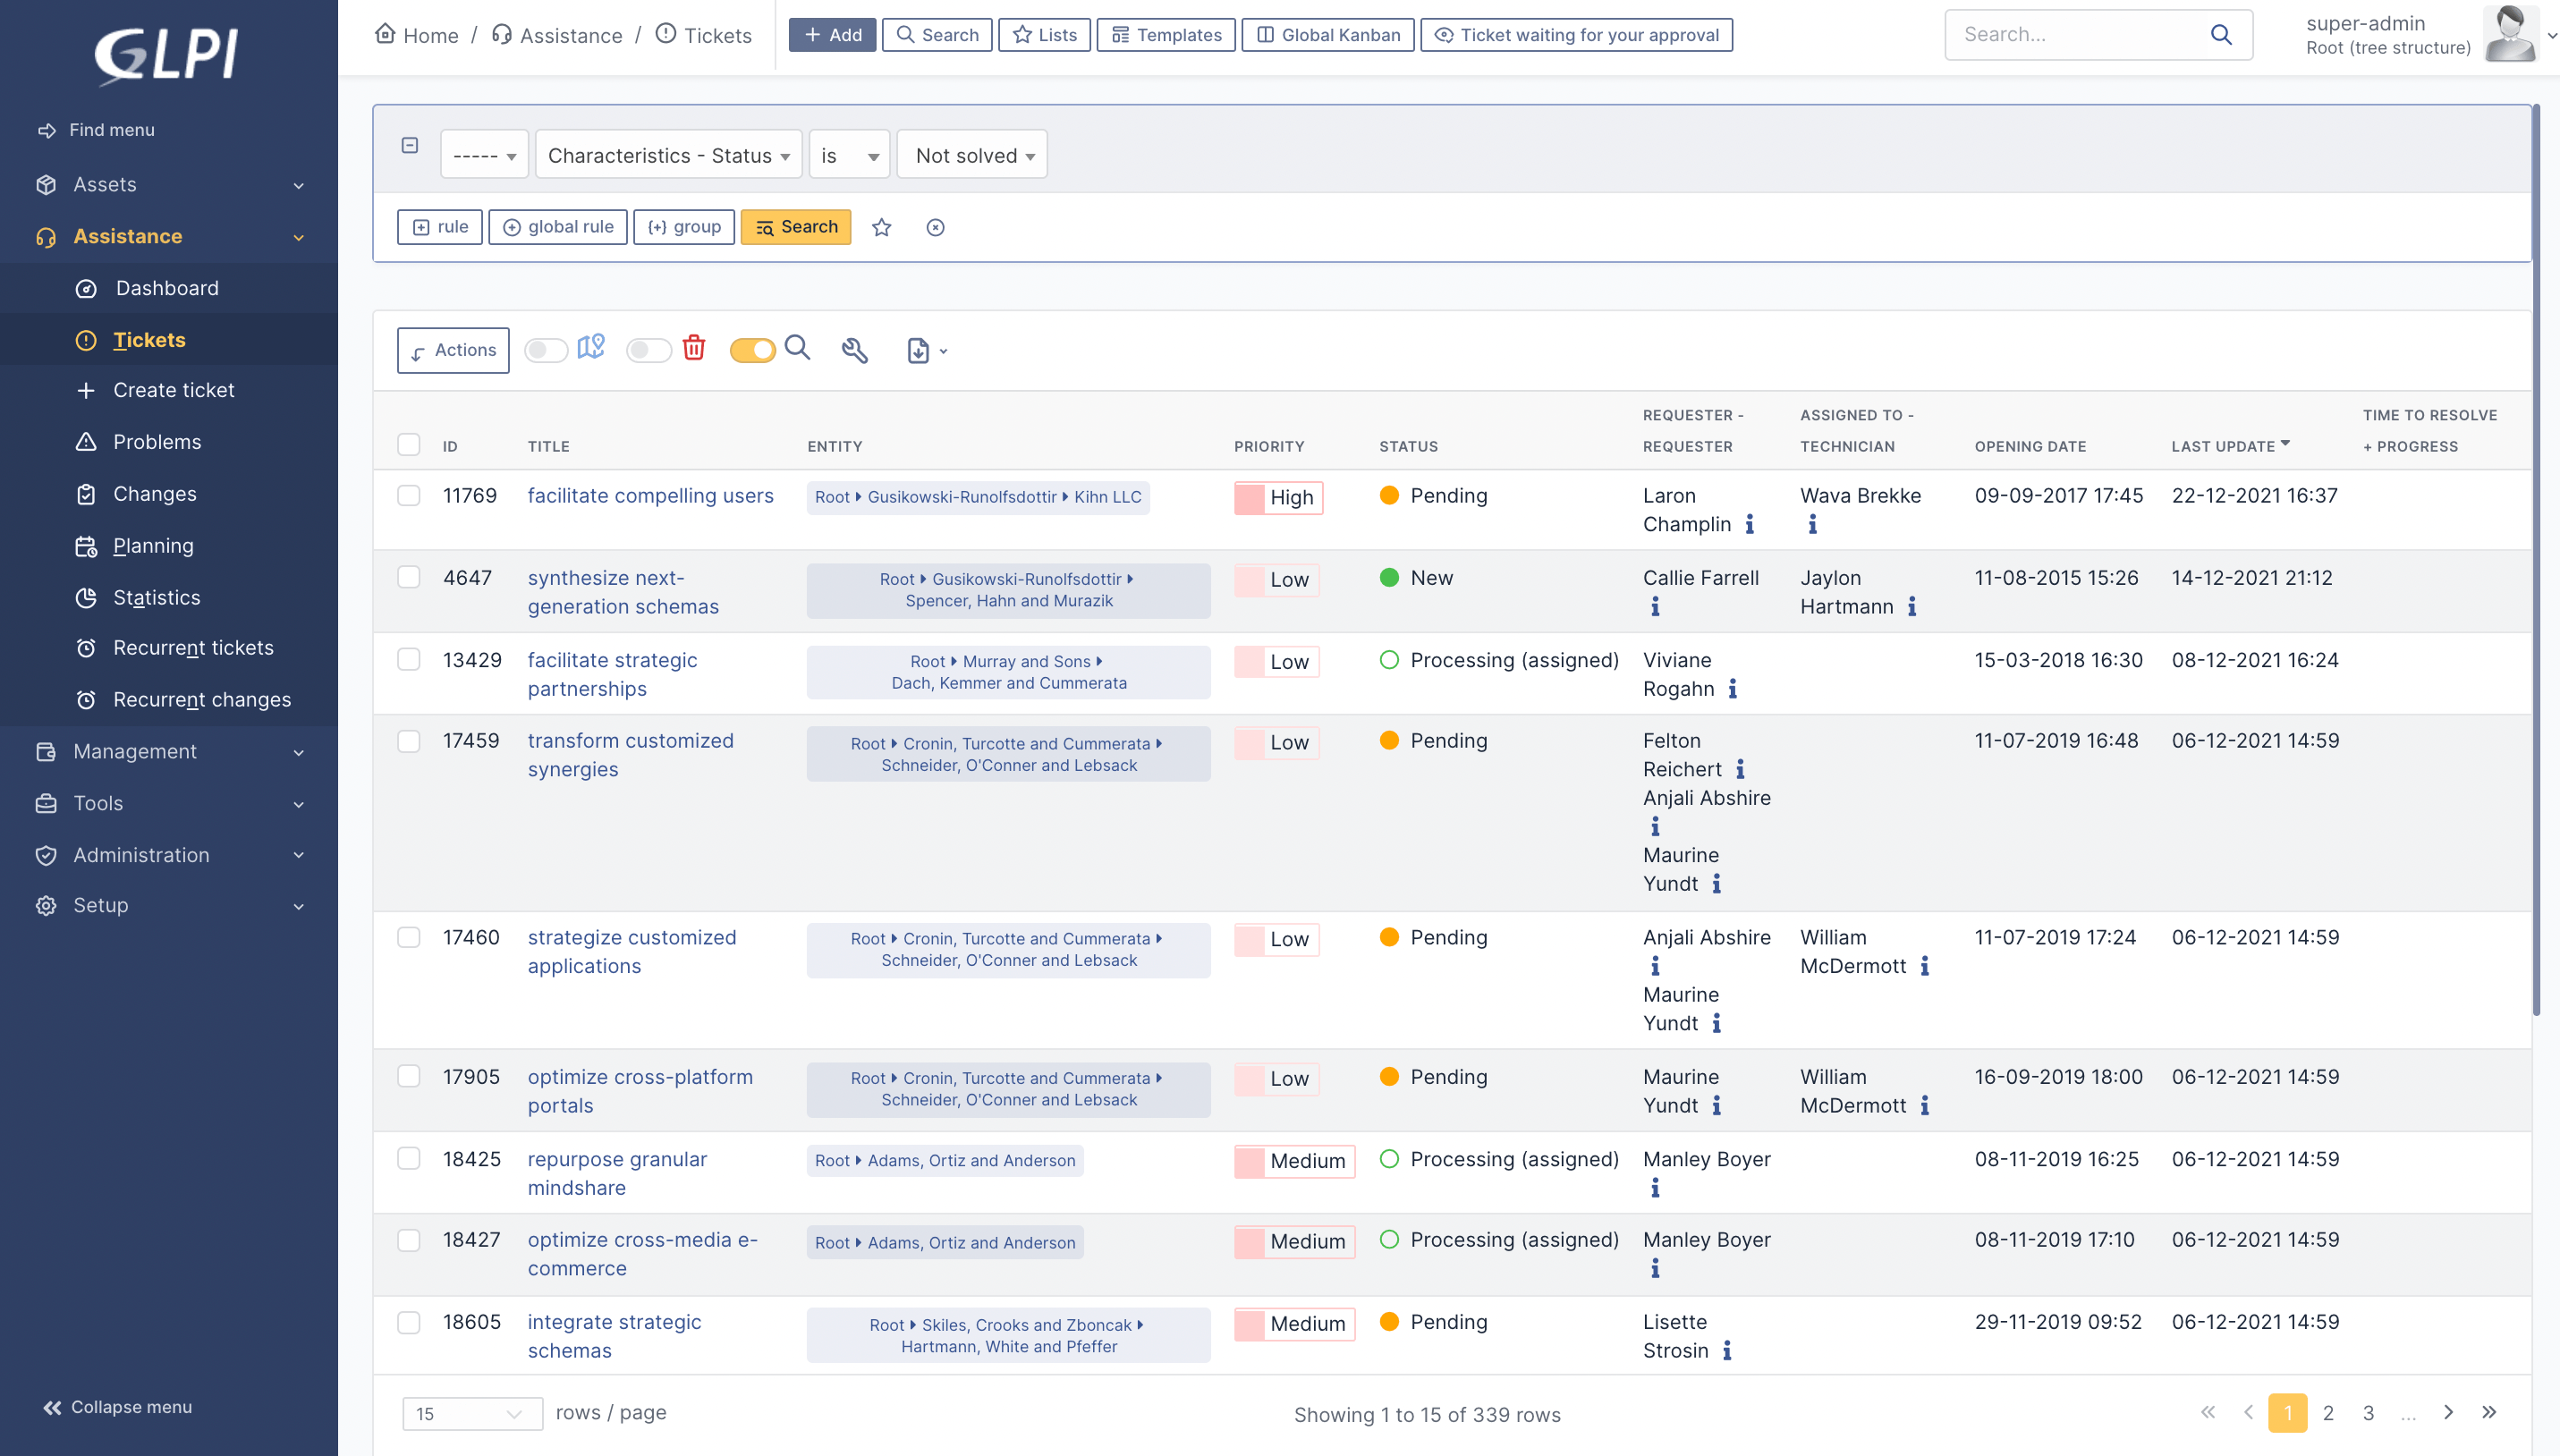
\includegraphics[width=0.7\textwidth,keepaspectratio]{Images/GLPI.png}
                            \caption{Interface de GLPI }
                            \label{fig:GLPI}
                        \end{figure}
  \vspace{0.4cm}
                  \noindent  --\hspace{0.5cm}  \textbf{Freshdesk}\par\smallskip
Freshdesk, créée en 2011 par Freshworks, s’impose comme une plateforme \textbf{SaaS} (\textit{Software as a Service}) de support client omnicanale capable de traiter les messages email, chat et réseaux sociaux tout en orchestrant une distribution intelligente des tickets et en enrichissant les interactions grâce à l'\textbf{IA} (\textit{Intelligence Artificielle}) Freddy AI. Cette solution conjugue la gestion des demandes, le suivi des SLA et l’automatisation des workflows pour améliorer la réactivité des équipes. Son modèle économique repose sur un principe freemium, avec un tarif de base à partir de 15~€/agent/mois et des options payantes pour des fonctionnalités avancées. \cite{freshdesk}                   
                    \begin{figure}[H]
                                        \centering
                            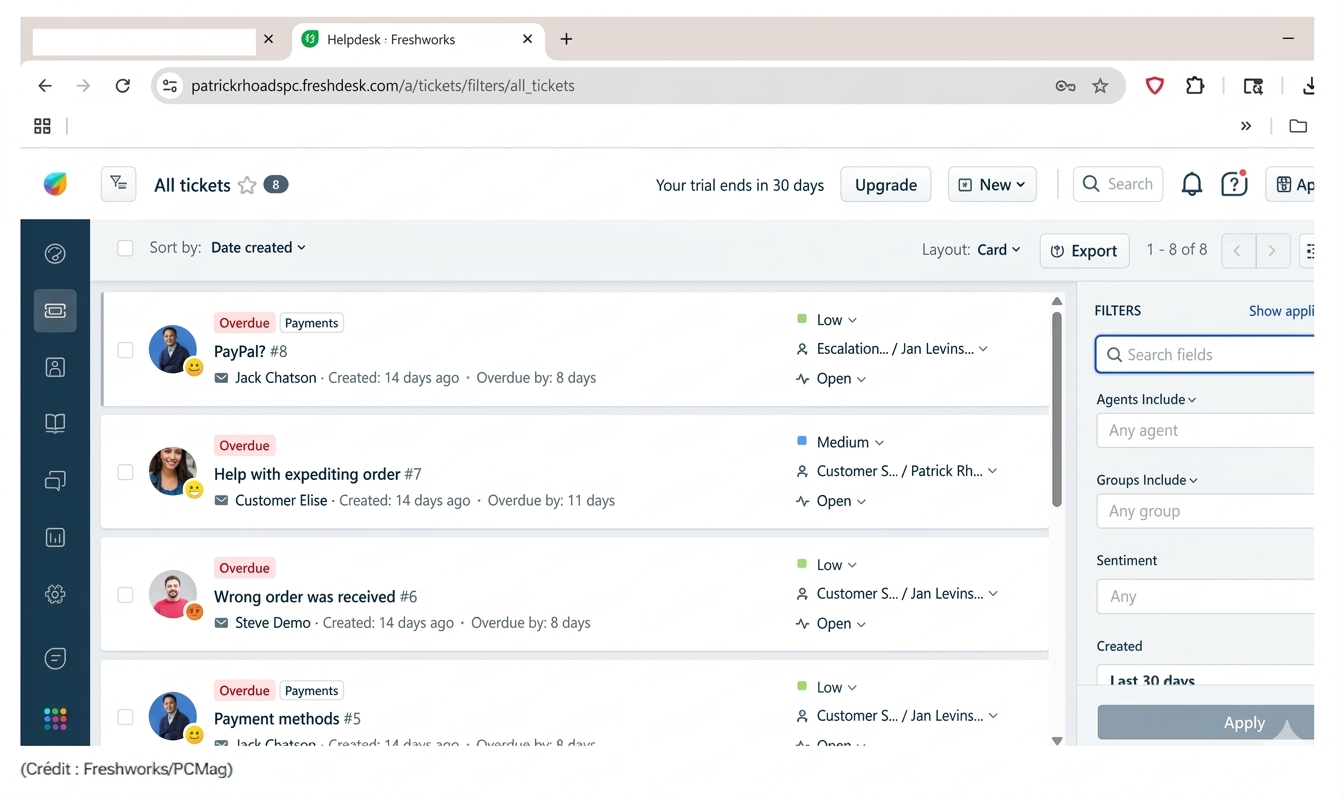
\includegraphics[width=0.7\textwidth,keepaspectratio]{Images/FreshDesk.png}
                            \caption{Interface de Freshdesk}
                            \label{fig:freshdesk}
                        \end{figure}
 \vspace{0.4cm}
                  \noindent --\hspace{0.5cm}  \textbf{Jira Service Management (Atlassian)}\par\smallskip
Jira Service Management, lancé en 2013 par Atlassian, propose un cadre ITSM (Information Technology Service Management) centré sur la gestion des incidents, des demandes et des changements, avec des tableaux de bord dédiés au suivi des engagements de service et des automatisations pour fluidifier les processus. Cette offre tire parti de l'écosystème Jira pour relier opérationnel et développement, ce qui facilite le pilotage des équipes et des actifs. Elle est distribuée principalement via un modèle d'abonnement \textbf{SaaS} (\textit{Software as a Service}), avec des versions cloud et des licences self-hosted pour les organisations qui préfèrent héberger leur solution en interne. \cite{jira-service-management}                    
                    \begin{figure}[H]
                        \centering
                        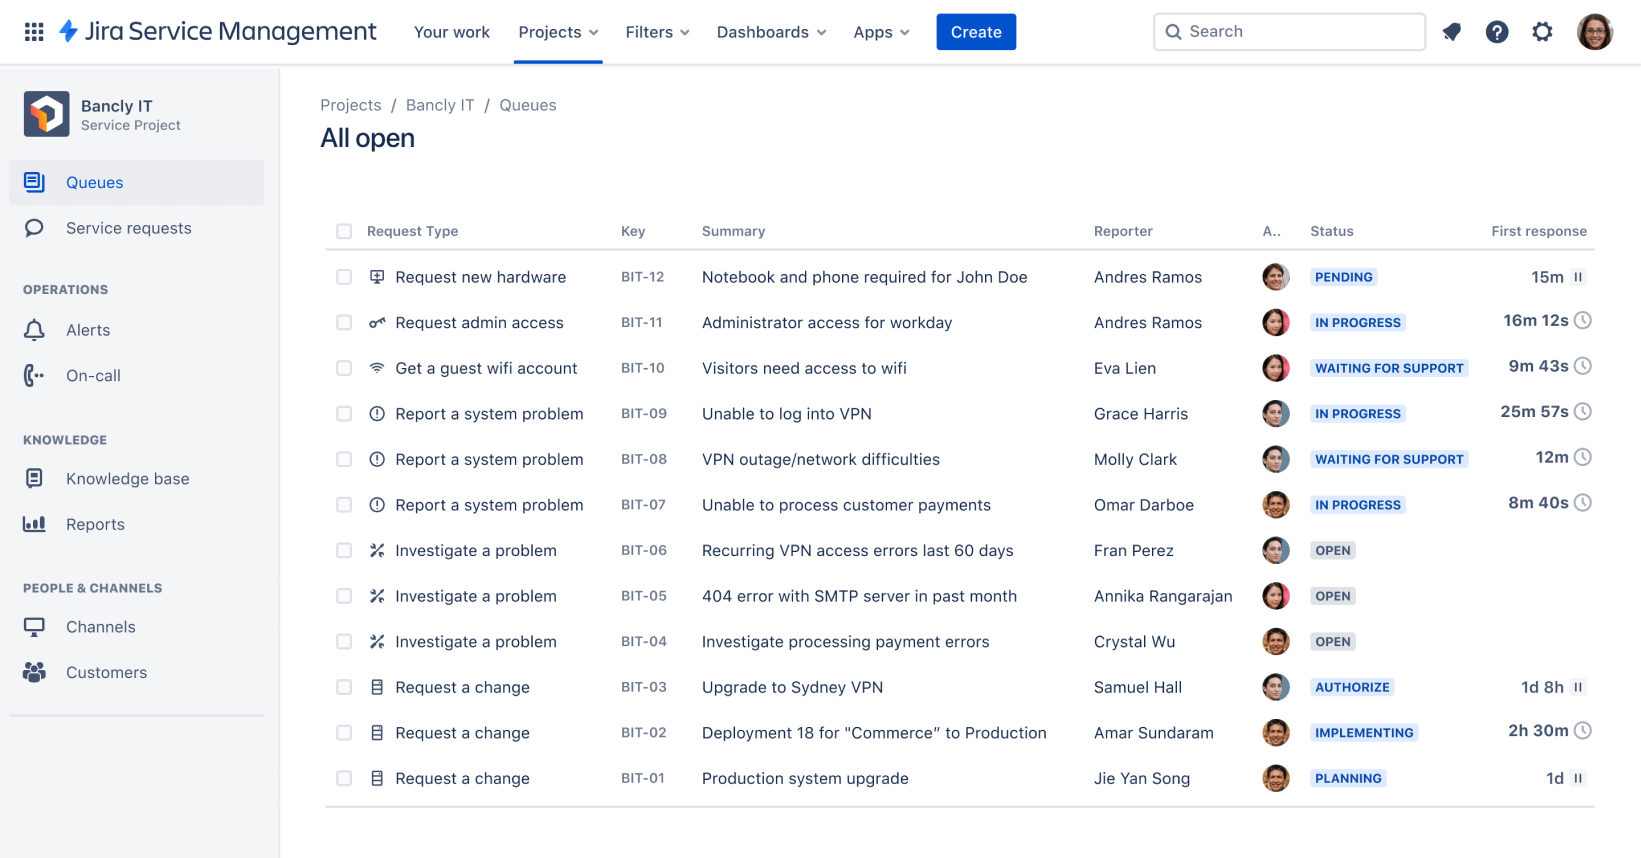
\includegraphics[width=0.7\textwidth,keepaspectratio]{Images/appJira.png}
                        \caption{Interface de Jira Service Management}
                        \label{fig:jira}
                    \end{figure}
            \noindent
\end{enumerate}


\subsubsection{Critique de l'existant}

Actuellement, la gestion des contrats de maintenance au sein de SolidWall Consulting repose sur un ensemble d'outils disparates : des documents Word pour les contrats, WhatsApp ou des courriels pour les demandes clients, et des fichiers Excel pour le suivi des interventions, sans système centralisé. Cette approche présente certaines limites.
\begin{enumerate}[label=\textcolor{bleuPerso}{\alph*)}, labelsep=0.5em]

 \item \noindent{\textbf{\textcolor{bleuPerso}{Limitations du processus actuel }}}
    \begin{itemize}[label=\ding{109}]
    \item \textbf{processus fragmenté : } La communication via e-mail fragmente la gestion. Les informations étant dispersées, le suivi des composants manquants devient complexe.  En l’absence de structure centralisée, il devient difficile de retrouver l'historique complet d'une intervention.
    \item \textbf{Absence de traçabilité :} L'absence de système de traçabilité rend le suivi des interventions difficile. Cela peut entraîner une perte de visibilité sur leur état, en cas de conflit avec un client ou lors d'un audit interne, ce qui représente un risque pour la crédibilité et la fiabilité de la société.
    \item \textbf{Risque de perte d'informations :} En raison de la fragmentation des processus, il existe un risque accru de perte d'informations importantes. Les documents sont stockés de manière non structurée, ce qui rend leur suivi et leur consolidation difficiles.
     \item \textbf{Complexité de la communication : } la communication au sein de l’équipe et avec les clients repose sur des échanges dispersés (courriels, messages), ce qui rend le flux des demandes peu clair et entraîne des retards dans le traitement des interventions.
    
    \end{itemize}

 \item \noindent{\textbf{\textcolor{bleuPerso}{Limitations des solutions existantes }}}
    \begin{itemize}[label=$\bullet$]
    \item \noindent\textbf{Complexité d'utilisation et courbe d'apprentissage}
    
    Les solutions existantes présentent une complexité d'usage importante. GLPI nécessite une formation de 2 à 3 jours pour les administrateurs avec une interface peu intuitive. Jira Service Management requiert une connaissance approfondie de l'écosystème Atlassian, créant une dépendance technique majeure.
    \newpage
    \item \noindent\textbf{Coût des licences et investissement financier}
    
    L'investissement financier représente un obstacle majeur pour l'adoption des solutions existantes. Les tarifs varient considérablement selon les offres : Freshdesk propose ses offres payantes à partir de 15€ par agent et par mois, tandis que Jira Service Management est tarifé à 20~€/agent/mois. GLPI, bien que gratuit en version communautaire, nécessite un minimum de 1500€ par an pour accéder au support entreprise. Pour une équipe de 10 utilisateurs, le coût annuel total s'élève ainsi à 1800€ pour Freshdesk, 2400€ pour Jira Service Management et 1500€ pour GLPI avec support.
    
    \item \noindent\textbf{Dépendance aux extensions et problèmes d'intégration}
    
    Les solutions du marché souffrent d'une architecture modulaire générant des coûts cachés. De nombreuses fonctionnalités avancées nécessitent des extensions payantes supplémentaires. Les mises à jour engendrent des problèmes de compatibilité, et l'intégration avec des systèmes existants nécessite souvent des développements spécifiques onéreux.
    \end{itemize}
\end{enumerate}
\subsubsection{Tableau comparatif des solutions}
\begin{table}[H]
    \centering
    \renewcommand{\arraystretch}{1.4}
    \arrayrulecolor{gray!70}
    \rowcolors{2}{gray!5}{white}
    \small
    \begin{tabularx}{\textwidth}{|>{\raggedright\arraybackslash}p{4cm}|>{\centering\arraybackslash}X|>{\centering\arraybackslash}X|>{\centering\arraybackslash}X|}
    \hline
    \rowcolor{blue!20}
    \textbf{Critères de comparaison} & \textbf{GLPI \cite{glpi}} & \textbf{Jira SM \cite{jira-service-management}} & \textbf{Freshdesk \cite{freshdesk}} \\
    \hline
    Gestion des tickets & \checkmark & \checkmark & \checkmark \\
    \hline
    Gestion des contrats \& SLA & Limité & Limité & $\times$ \\
    \hline
    Gestion de parc (Assets) & \checkmark & Limité (Payant) & $\times$ \\
    \hline
    Messagerie \& Chat intégré & Limité & Limité & \checkmark \\
    \hline
    IA \& Suggestions automatiques & $\times$ & \checkmark & \checkmark \\
    \hline
    Application \& Accès Mobile & Limité & \checkmark & \checkmark \\
    \hline
    Facilité d'utilisation & Moyenne & Moyenne & Facile \\
    \hline
    Coût indicatif (10 users / an) & 1500 € & 2400 € & 1800 € \\
    \hline
    \end{tabularx}
    \caption{Analyse comparative des solutions de gestion de maintenance du marché}
    \label{tab:comparaison_solutions}
\end{table}
\newpage
\smallskip
\noindent\textit{\textbf{Remarque sur les coûts} — Les tarifs annuels présentés pour 10 utilisateurs correspondent aux offres de base : 1~800~€/an pour Freshdesk, 2~400~€/an pour Jira SM, et 1~500~€/an pour le support entreprise de GLPI (dont la version communautaire reste gratuite). Ces montants excluent les fonctionnalités optionnelles, les supports premium et les frais de personnalisation.}
\subsubsection{Solution proposée}

C'est dans ce cadre que s'inscrit \textbf{SolidMaint}, une 
plateforme web intégrée visant à automatiser et à centraliser 
l'ensemble du processus de gestion des contrats de maintenance 
au sein de \textbf{SolidWall Consulting}. Elle s'articule 
autour de trois modules fonctionnels complémentaires :

\noindent\textbf{Module 1 : Gestion des Clients, Projets et Contrats}

Ce module centralise la gestion des clients, des projets et 
des contrats de maintenance. Il offre une visibilité complète 
sur les engagements contractuels par client et intègre un 
système d'alertes préventives permettant d'anticiper les 
échéances et de garantir le respect des accords de niveau 
de service (SLA).

\noindent\textbf{Module 2 : Gestion des Demandes et Tickets}

Ce module structure le cycle de vie complet des demandes 
clients, depuis leur soumission jusqu'à leur clôture. Il 
automatise la génération des tickets, facilite leur 
affectation aux développeurs compétents et assure un suivi 
précis du temps d'intervention, contribuant ainsi à une 
meilleure maîtrise des délais de résolution.

\noindent\textbf{Module 3 : Collaboration et Assistance 
Intelligente}

Ce module regroupe les fonctionnalités avancées de 
communication et d'intelligence artificielle, notamment 
la messagerie en temps réel, la gestion documentaire et 
les notifications multicanaux, afin de fluidifier les 
échanges entre les différents acteurs de la plateforme.

En réponse aux insuffisances identifiées, \textbf{SolidMaint} 
centralisera l'ensemble des processus de maintenance au sein 
d'un environnement unifié, fiable et évolutif, permettant à 
\textbf{SolidWall Consulting} d'améliorer sa réactivité et 
de renforcer la qualité de ses prestations.

\section{Choix du framework de gestion de projet}
\label{sec:methodologie}
Le choix méthodologique est déterminant pour la réussite d'un projet de développement. Une méthodologie appropriée structure le travail, optimise la gestion des ressources et garantit la qualité du livrable dans le respect des délais impartis.

\subsection{Méthodologie classique }
La méthodologie classique s'appuie sur une planification prédictive et une exécution séquentielle : chaque phase est définie au préalable, puis réalisée de l'analyse des besoins à la mise en production. Cette stratégie offre une maîtrise élevée des livrables, des délais et des coûts lorsque les exigences sont stables et que le périmètre évolue peu.

Cependant, cette rigidité expose le projet à des retours en arrière coûteux dès qu'une correction ou un nouveau besoin apparaît après la conception. Le cycle en V met en lumière cette logique en associant systématiquement chaque phase de conception à une phase de validation, ce qui privilégie la conformité au détriment de l'adaptabilité.\cite{brandenbourg-gestion}

\subsubsection{Principes de la méthodologie classique}
L'approche repose sur une progression linéaire où chaque étape sert de fondation à la suivante. Elle exige une définition détaillée des besoins en phase initiale et une validation formelle à chaque transition, ce qui limite la capacité d'adaptation en cas de changement ultérieur.



\subsection{Méthodologie Agile}
L'approche agile s'appuie sur une progression itérative et sur l'apprentissage continu. Plutôt que de figer l'ensemble du périmètre en début de projet, elle privilégie des cycles de travail courts qui permettent de valider des fonctionnalités opérationnelles et de réajuster les priorités selon les retours métiers. Cette dynamique permet au projet de rester proche des attentes des utilisateurs et de limiter les écarts entre les besoins réels et les livrables.

Dans le contexte de SolidMaint, l'agilité renforce la capacité à intégrer rapidement de nouvelles demandes ou des corrections, tout en maintenant un rythme de livraison régulier. Ce mode de travail favorise une collaboration étroite entre l'équipe de développement, le Product Owner et les parties prenantes, et transforme le changement en levier  \newline d'amélioration plutôt qu'en source de retard. \cite{agile-manifesto}




\subsubsection{Choix de l’approche Agile}
Le domaine de la maintenance impose des besoins imprévisibles, excluant toute planification rigide. Nous adoptons donc une approche agile basée sur la simplicité afin de produire l'essentiel efficacement. Pour cela, nous avons choisi la méthode Scrum, qui s'impose comme le cadre itératif idéal pour livrer rapidement de la valeur tout en restant réactifs aux changements.
\subsubsection{ Les principales méthodes Agiles}
Le tableau suivant met en évidence les méthodes Agile les plus couramment utilisées, selon différents critères de comparaison.
\begin{table}[H]
    \centering
    \renewcommand{\arraystretch}{1.6} % Espace vertical pour aérer les cellules
    
    % Couleur des bordures et alternance des couleurs de lignes
    \arrayrulecolor{gray!70}      
    \rowcolors{2}{gray!5}{white} 
    
    \begin{tabularx}{\textwidth}{
        | >{\bfseries\raggedright\arraybackslash}p{3.5cm} 
        | >{\centering\arraybackslash}X 
        | >{\centering\arraybackslash}X 
        | >{\centering\arraybackslash}X 
        | }
        
    \hline
    \rowcolor{blue!20} \textbf{Critères} & \textbf{Scrum} & \textbf{Kanban} & \textbf{Extreme Programming (XP)} \\
    \hline
    Type de projet & Incrémental & Continu & Technique \\
    \hline
    Critère d'évaluation & Vélocité & Fluidité & Qualité \\
    \hline
    Gestion des risques & Détection & Visualisation & Prévention \\
    \hline
    Implication client & Ponctuelle & Variable & Très forte et continue \\
    \hline
    
\end{tabularx}
    \vspace{0.2cm}
    \caption{Les principales méthodes Agiles.}
    \label{tab:methodes_agiles}
\end{table}

\subsubsection{Choix de la méthode Scrum}
Scrum a été retenue comme cadre de travail pour structurer le développement en itérations courtes tout en s'adaptant aux changements fréquents. Cette méthode offre plusieurs avantages décisifs :
\newline
\noindent
         --\hspace{0.5cm} Collaboration continue entre l'équipe et les parties prenantes
\newline --\hspace{0.5cm}  Adaptation rapide aux changements grâce aux cycles itératifs
\newline --\hspace{0.5cm} Livraisons régulières de fonctionnalités opérationnelles
\newline --\hspace{0.5cm} Détection précoce des problèmes et ajustements immédiats
\newline --\hspace{0.5cm} Transparence totale sur l'avancement du projet

\begin{figure}[H]
        \centering
        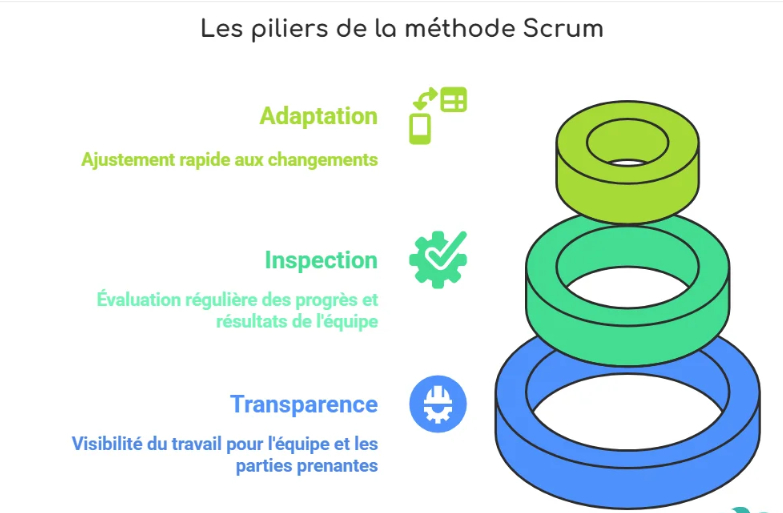
\includegraphics[width=0.7\textwidth,keepaspectratio]{Images/les piliers de la methodologie.png}
        \caption{les piliers de la méthode Scrum}
        \label{fig:les piliers de la méthode Scrum}
\end{figure}

\subsection{Fondements de SCRUM }
Scrum est un cadre organisationnel qui structure le développement itératif par successifs cycles courts appelés sprints, généralement étalés sur 2 à 4 semaines. Ce modèle s'appuie sur l'expression des besoins sous forme d'items de travail (user stories) ordonnancés et priorisés, permettant une livraison régulière de valeur métier mesurable et exploitable. La philosophie sous-jacente vise à concilier productivité de l'équipe et satisfaction continue du client par l'ajustement perpétuel. 

Scrum repose sur trois piliers fondamentaux qui constituent sa colonne vertébrale : la \textbf{transparence} crée une visibilité partagée et incontestable sur la progression réelle du travail, les risques et les décisions ; l'\textbf{inspection} encourage l'évaluation critique et régulière des artefacts (produit, processus, incrément) pour identifier rapidement tout écart ou opportunité ; enfin, l'\textbf{adaptation} autorise l'équipe à réviser son approche, ses priorités et ses méthodes en réaction directe aux faits observés et aux retours des parties prenantes.\cite{scrum-guide}

\subsection{Rôles de SCRUM}
La structure organisationnelle de Scrum s'appuie sur trois rôles qui répartissent clairement les responsabilités entre le pilotage métier, la facilitation du cadre et la réalisation technique.

\subsubsection{Product Owner}
Le Product Owner est responsable de la valeur métier du produit et de la vision métier du projet. Il définit les exigences de l’application et priorise les éléments du Product Backlog en fonction des objectifs de la société.
\subsubsection{Scrum Master}
Le Scrum Master est le garant du cadre Scrum. Il veille à ce que les pratiques agiles soient respectées, facilite les événements et aide à lever les obstacles qui freinent l’équipe.
\subsubsection{Les développeurs}
L’équipe de développement est chargée de la réalisation opérationnelle : conception, configuration,
développement et tests. Elle transforme les besoins priorisés en incréments fonctionnels prêts à être validés.

\subsection{Événements Scrum}
Les événements Scrum constituent des points de synchronisation structurés qui rythment l'exécution, entretiennent la discipline itérative, et incarnent les trois piliers de transparence, d'inspection et d'adaptation. Chaque événement possède une durée maximale prescrite et sert un objectif métier bien défini.
\begin{itemize}[nosep, left=0pt, label=\textbullet]
\item \textbf{Sprint~:} Conteneur itératif d'une durée fixe (généralement 2 à 4 semaines) au cours duquel l'équipe s'engage à livrer un incrément potentiellement commercialisable du produit. Chaque sprint débute par une planification et s'achève par une revue et une rétrospective.
\item \textbf{Sprint Planning~:} Événement de lancement où l'équipe et le Product Owner se rencontrent pour définir l'objectif du sprint et sélectionner les éléments du Product Backlog jugés réalisables. Cet atelier établit le Sprint Backlog et fixe les attentes de livrables.
\item \textbf{Daily Scrum (ou Mêlée quotidienne)~:} Synchronisation brève de 15 minutes maximum où l'équipe revient sur ses accomplissements, anticipe les travaux prévus et signale les obstacles rencontrés. Cet instant de transparence quotidienne renforce cohésion et réactivité.
\item \textbf{Sprint Review~:} Présentation et démonstration du travail accompli durant le sprint devant les parties prenantes. Elle permet la collecte de retours formels et l'ajustement du Product Backlog selon les commentaires et les besoins révisés.
\item \textbf{Sprint Retrospective~:} Moment d'introspection où l'équipe analyse collectivement son fonctionnement, met en lumière réussites et difficultés, et décide d'actions concrètes pour l'amélioration continue des futurs sprints.
\end{itemize}

\subsection{Artéfacts Scrum}
Les artéfacts Scrum matérialisent et expriment le travail, la valeur livrée et l'avancement du projet. Ils constituent des vecteurs de transparence et de communication pour tous les acteurs.
\begin{itemize}[nosep, left=0pt, label=\textbullet]
\item \textbf{Product Backlog~:} Inventaire dynamique et ordonné de tous les besoins, fonctionnalités, corrections et tâches à réaliser. Maintenu et priorisé par le Product Owner selon retours clients et valeur métier, il évolue constamment et reflète l'état réel du produit visé.
\item \textbf{Sprint Backlog~:} Projection du Product Backlog pour le sprint en cours, sélectionné collectivement lors de la planification. Il formalise l'engagement de l'équipe sur les éléments à livrer et constitue la source unique de vérité pour le travail en cours.
\item \textbf{Incrément du Produit~:} Somme des éléments du Product Backlog finalisés au cours du sprint actuel et de tous les sprints précédents. Il représente une version cohérente, intégrée et testée du produit, offrant une valeur tangible et démontrée au destinataire. Seul un incrément répondant aux critères d'acceptation est comptabilisé.
\end{itemize}
\subsection{Cycle de vie}
    Le cycle de vie Scrum se compose de sprints successifs, chacun comprenant une planification, le développement, des réunions quotidiennes, une revue et une rétrospective. Ce processus itératif permet d'adapter le produit en continu aux besoins du client et d'améliorer l'équipe à chaque itération.

    \begin{figure}[H]
        \centering
        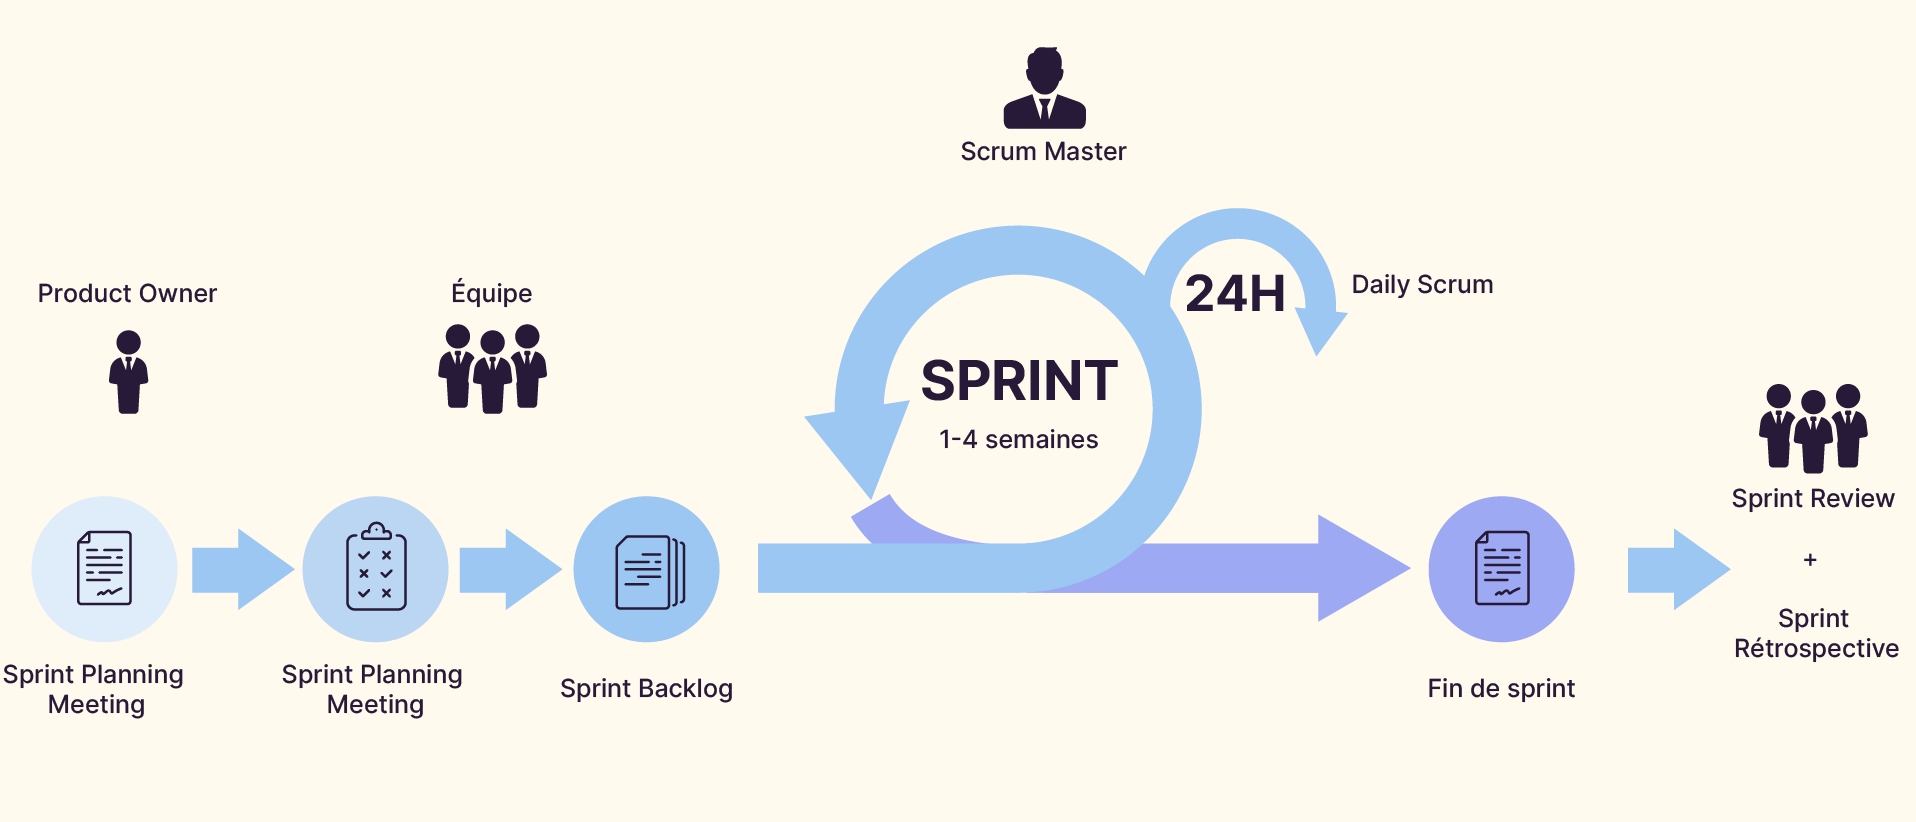
\includegraphics[width=0.75\textwidth,keepaspectratio]{Images/processus_scrum.png}
        \caption{Cycle de vie Scrum}
    \end{figure}
    
   
\section{Langage de modélisation UML}
« Le langage de modélisation unifié (UML) est un langage permettant de spécifier, visualiser, construire et documenter les artefacts des systèmes logiciels, ainsi que de modéliser des systèmes métier et d'autres systèmes non logiciels. L'UML représente un ensemble de bonnes pratiques d'ingénierie qui ont fait leurs preuves dans la modélisation de systèmes vastes et complexes. » \cite{omg-uml-importance}

\begin{figure}[H]
        \centering
        
\includegraphics[width=0.4\textwidth,keepaspectratio]{Images/UML.png}
        \caption{Logo UML}
    \end{figure}
    Pour concevoir notre application, nous avons choisi UML comme langage de modélisation. Ce choix s'appuie sur plusieurs points forts tels que la communication entre l'équipe et la cohérence architecturale qui se fait de manière simplifiée et standardisée.
\section*{Conclusion}
    Ce chapitre a établi le cadre général de notre projet \textbf{SolidMaint} en présentant l'organisme d'accueil SolidWall Consulting et en analysant les enjeux de la gestion des contrats de maintenance. L'étude critique de l'existant a révélé des limitations significatives dans les processus actuels, tandis que l'analyse comparative des solutions du marché a confirmé la pertinence de développer une solution sur mesure.
    La solution \textbf{SolidMaint} proposée répond à ces défis par une approche intégrée centralisant l'ensemble du cycle de vie des contrats. L'adoption de la méthodologie Scrum et la planification en quatre sprints garantissent une approche itérative et collaborative pour la réalisation du projet.
    \newline Le chapitre suivant détaillera la spécification des besoins et la modélisation de la solution.

